%
%
%
\subsection{Steady flow over a turbine rotor blade}
\label{VKI_LS59.subsec}
%
 The calculations presented in this Section are for the 2D Von Karman Institute gas
 turbine rotor blade (VKI LS59).
 This blade represents a challenging test for a transonic flow solver and
 it has been used by several researchers for code validation
 (Arnone and Swanson \citeyearNP{Arnone:2}).
 The flow is turned
 about $96\se{o}$ by the blade, with an exit Mach number which varies from 0.81
 up to 1.20. The blade passage is convergent and originally designed to work
 up to sonic conditions. In fact, the suction side is curved even after the throat
 region, which produces a strong trailing edge shock in transonic regimes.
 Kiock et al. \citeyear{Kiock:1} provide the geometry and
 detailed experimental data for this rotor blade.
%
\begin{figure}[ht]
 \centerline{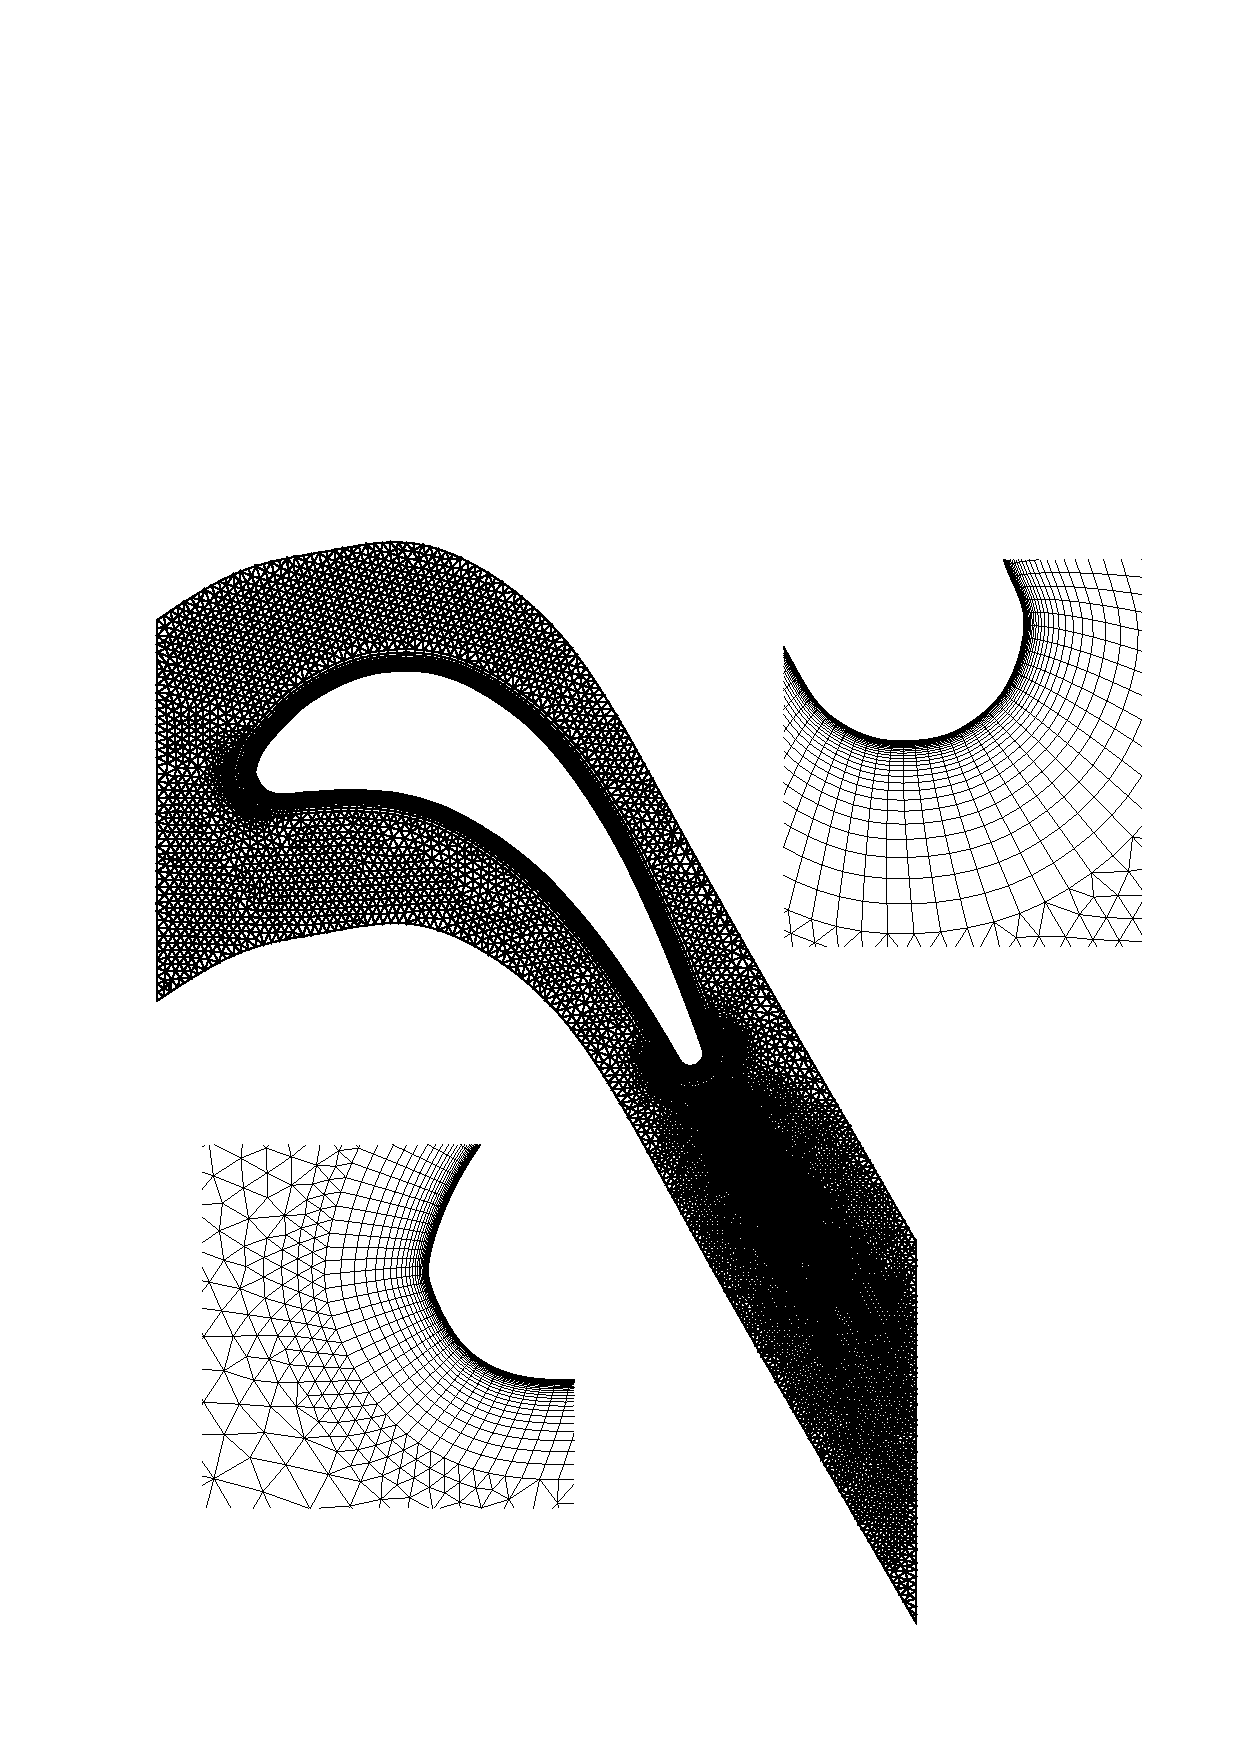
\includegraphics[width=110mm,clip=t]{CHAP_NONLIN/FIGURE/vki_mesh_1.pdf}}
 \caption{VKI LS59 rotor blade. Computational mesh with zoom views at leading- and
          trailing-edges}
 \label{vki_mesh_1.fig}
\end{figure}
%

 The inlet flow angle is $30\se{o}$ while the Reynolds number
 based on the blade chord and outlet conditions is in the range from
 $6.2\cdot10\se{5}$ up to $8.3\cdot10\se{5}$.
 A view of the computational mesh is shown in Fig. \ref{vki_mesh_1.fig}.
 This mesh contains 7,440 quadrilaterals in the boundary layer region and
 12,842 triangles in the rest of the domain which yields a total of 14,203 points.
%
%
\begin{figure}
 \begin{center}
  \begin{tabular}{ccc}
    \subfigure[Grid 2: 3587 cells]
       {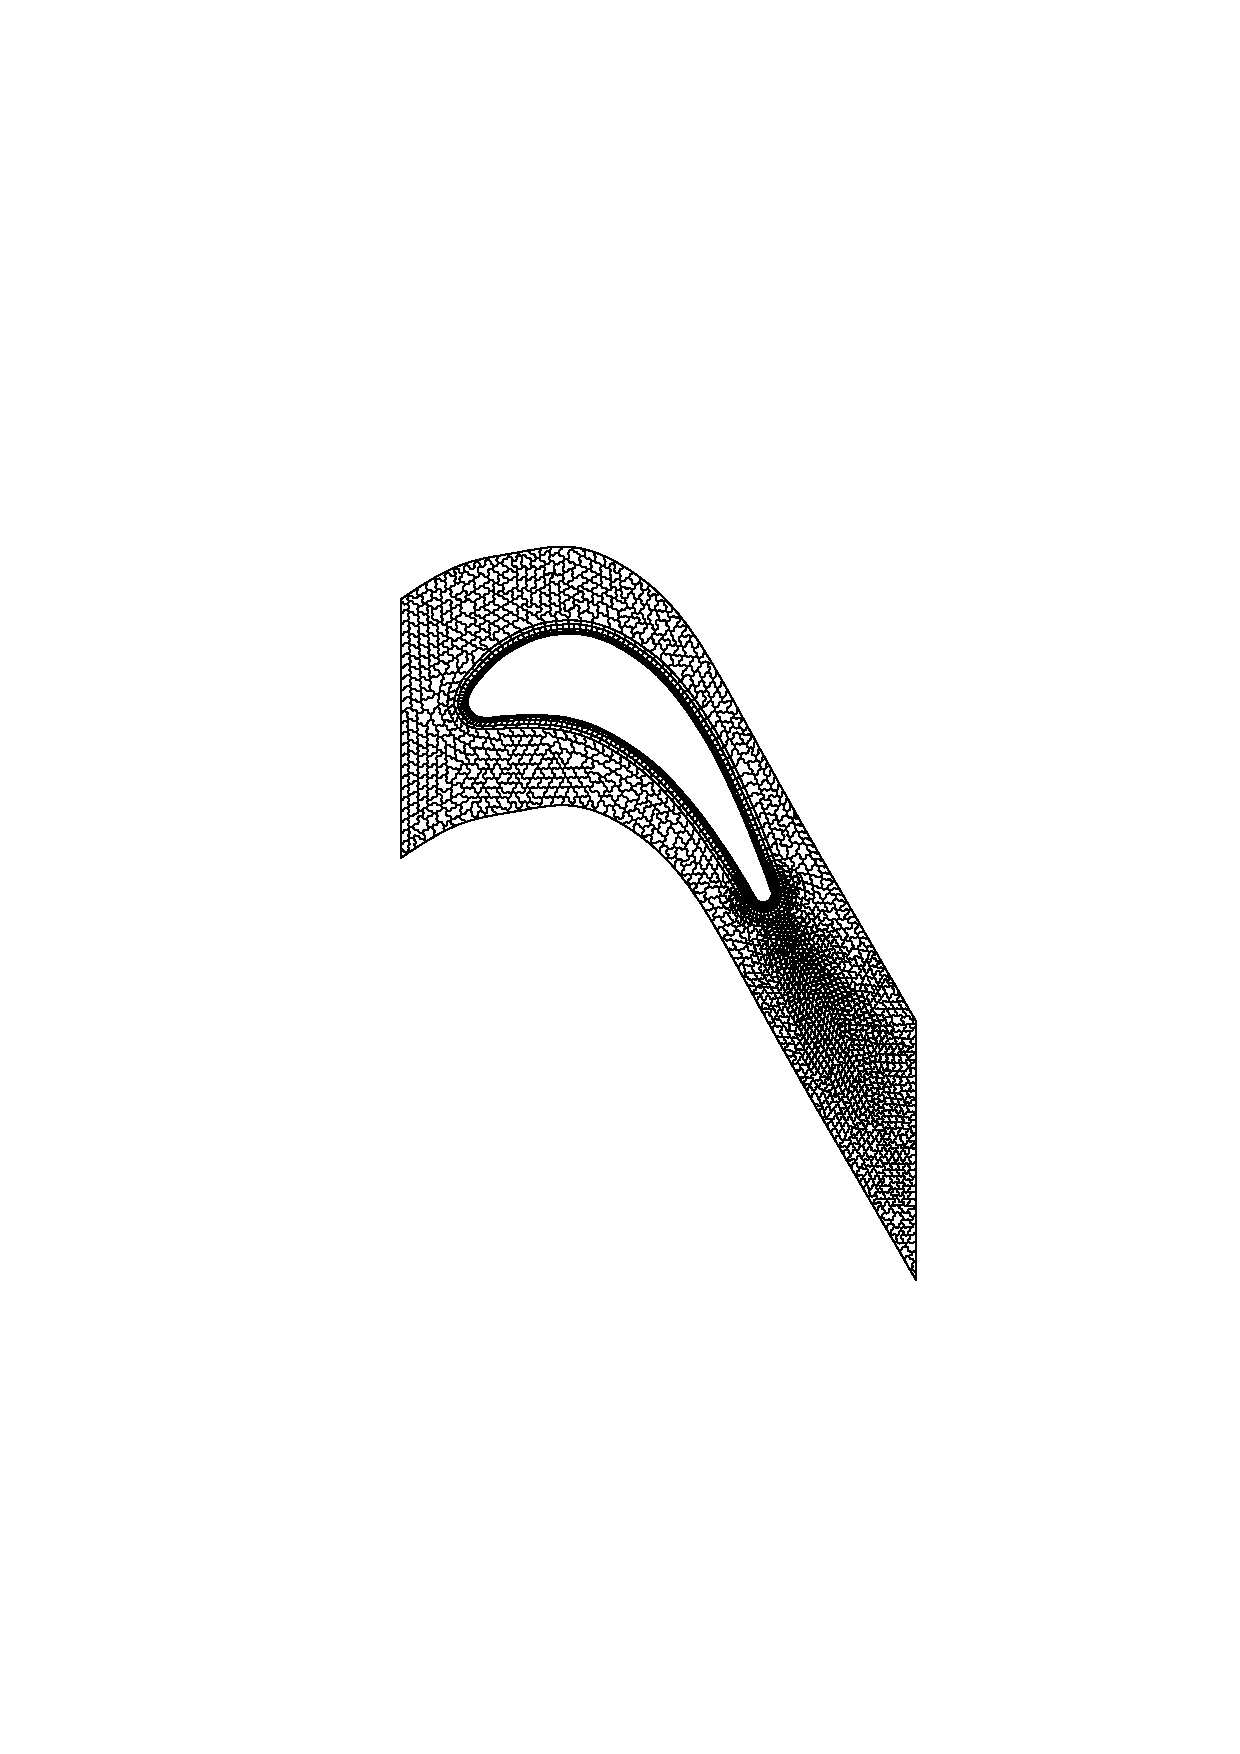
\includegraphics[width=45mm,clip=t]{CHAP_NONLIN/FIGURE/vki_mesh2.pdf}}
        &
    \subfigure[Grid 3: 908 cells]
       {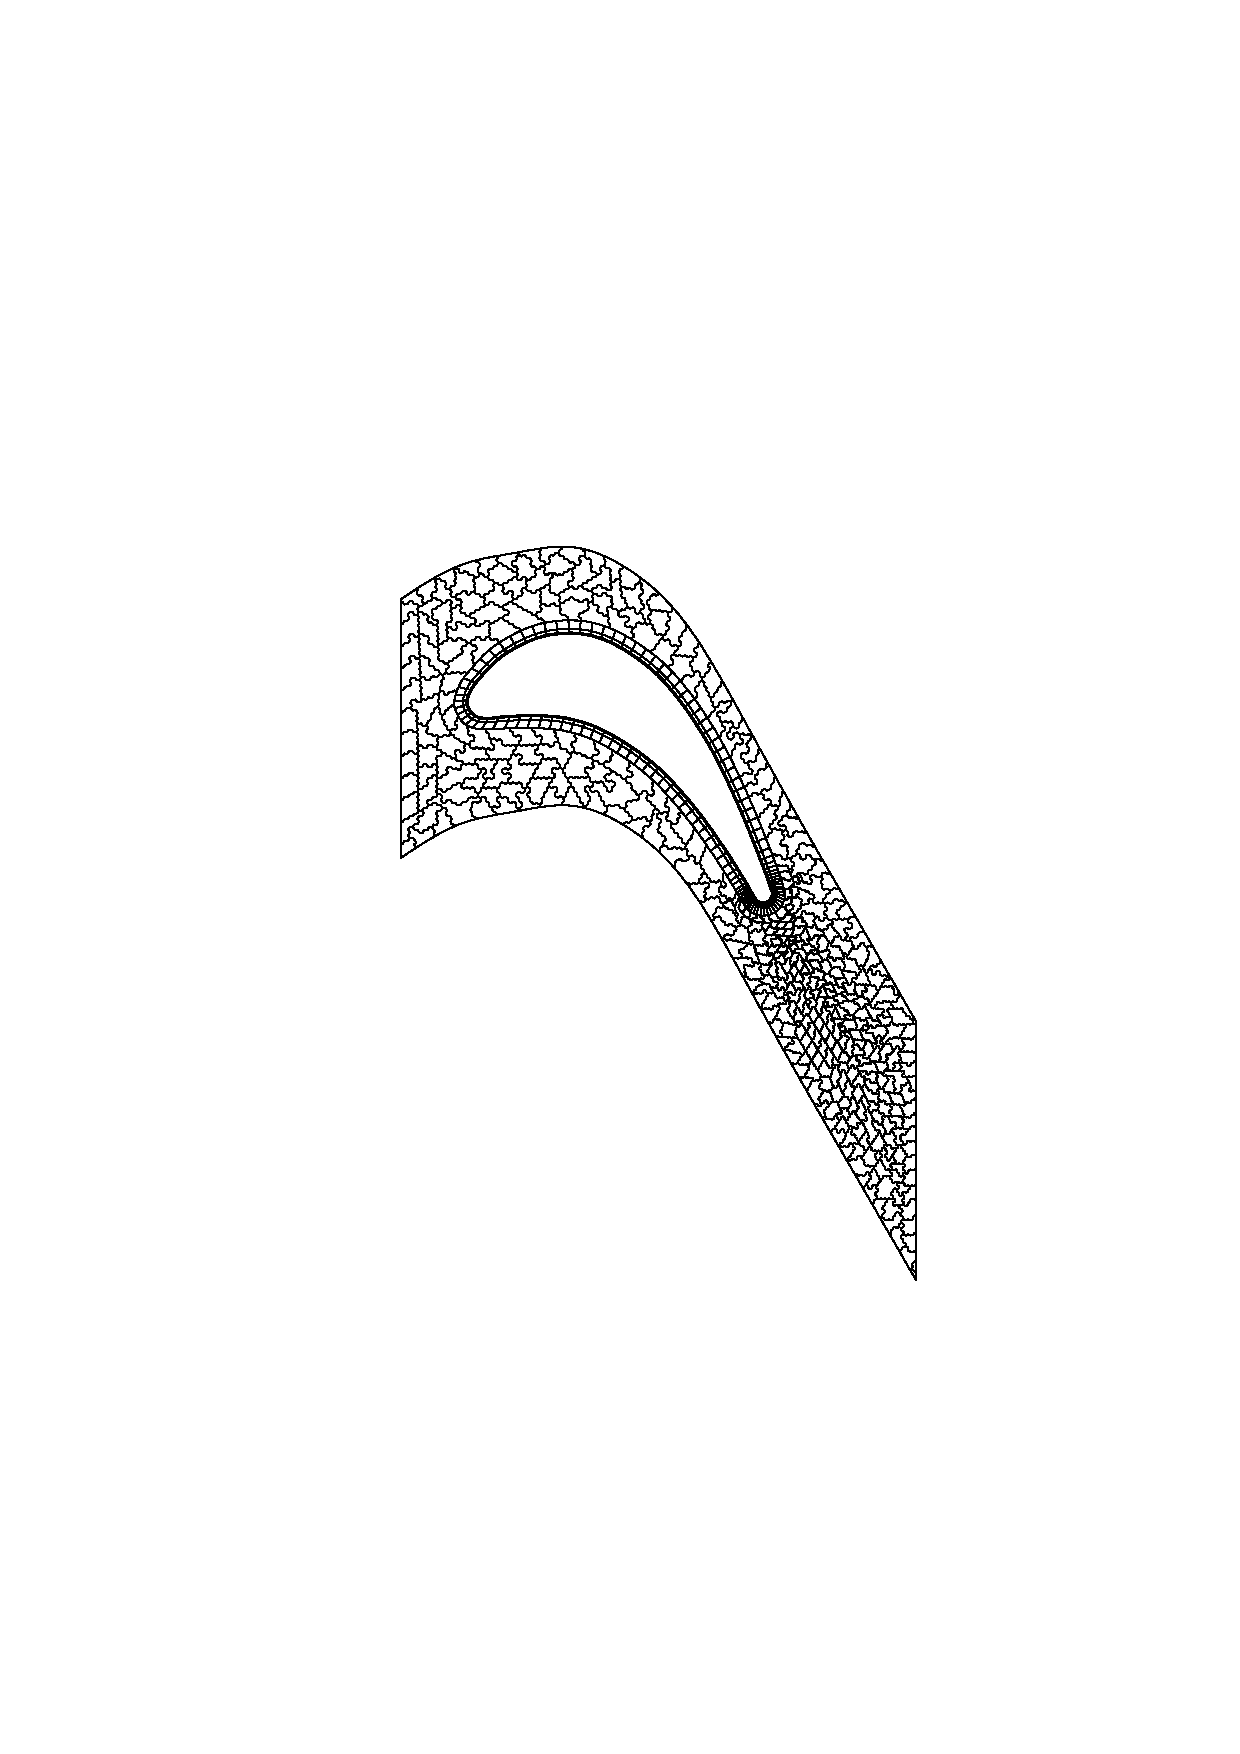
\includegraphics[width=45mm,clip=t]{CHAP_NONLIN/FIGURE/vki_mesh3.pdf}}
        &
    \subfigure[Grid 4: 239 cells]
       {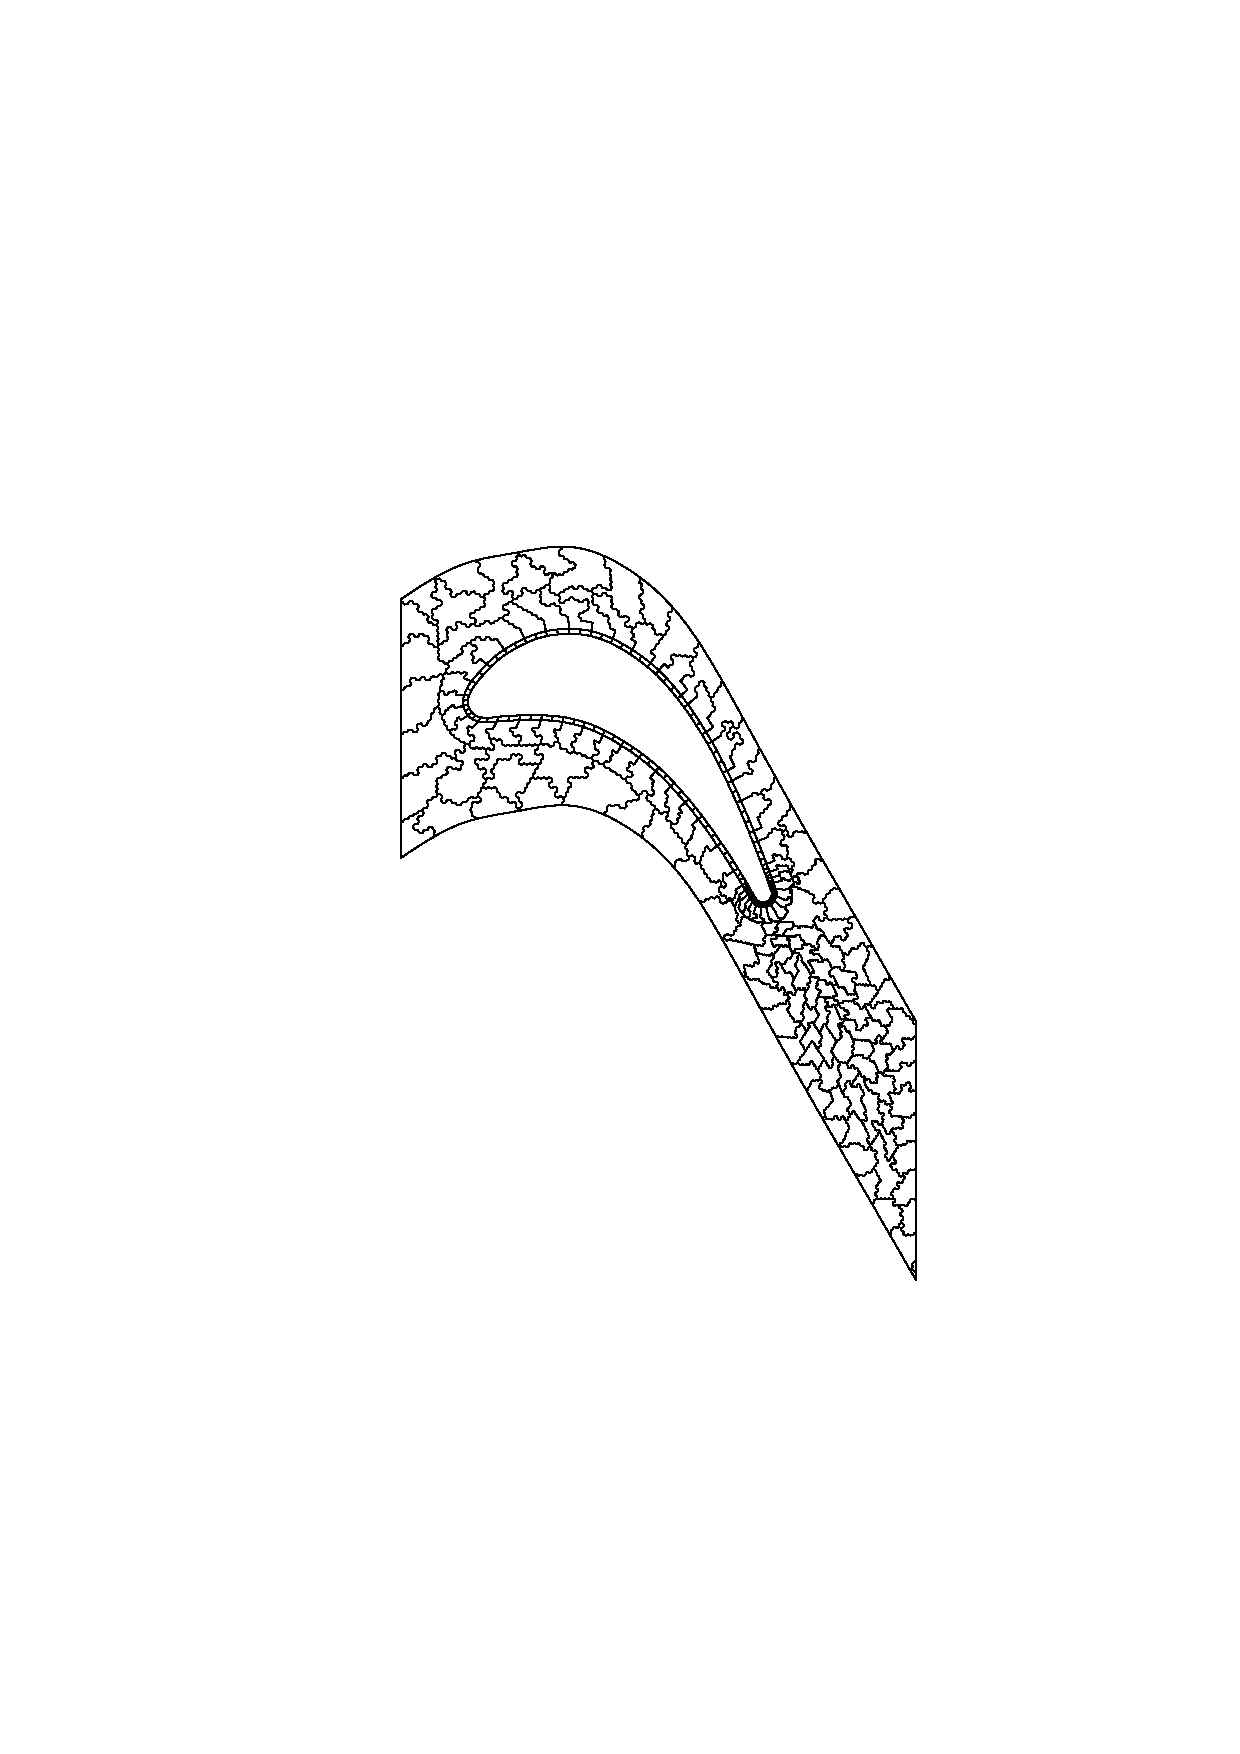
\includegraphics[width=45mm,clip=t]{CHAP_NONLIN/FIGURE/vki_mesh4.pdf}}
  \end{tabular}
 \end{center}
 \vspace{-5mm}
 \caption{VKI LS59 rotor blade. Agglomerated grids}
 \label{vki_agglo.fig}
\end{figure}
%
 Three succesively agglomerated meshes were used in a four grid W-type cycle
 in conjunction with the line-implicit preconditioner described
 in Appendix \ref{multigrid.chap}.
 Fig. \ref{vki_agglo.fig} shows the control volumes associated with
 these agglomerated grids.
%
\begin{figure}
  \centerline{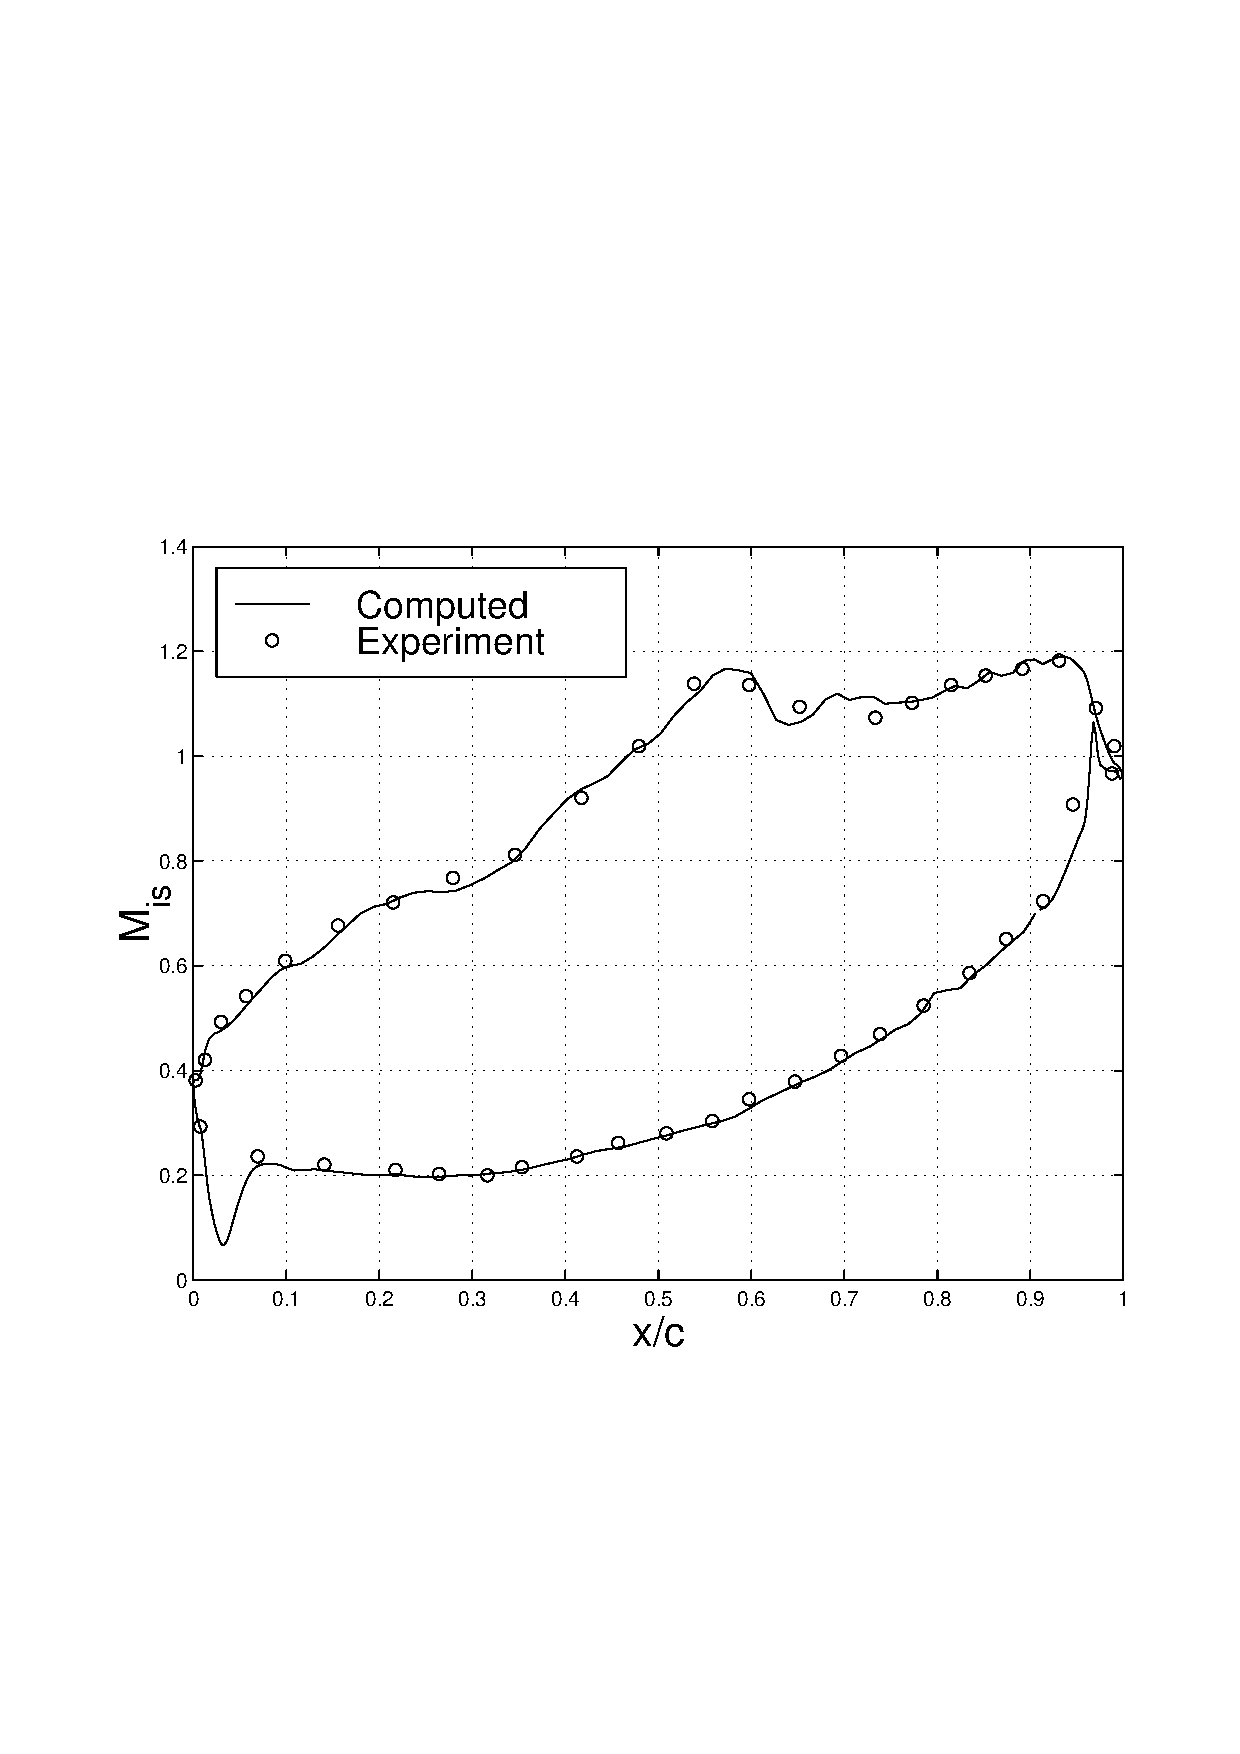
\includegraphics[width=130mm,clip=t]{CHAP_NONLIN/FIGURE/vki_blade.pdf}}
 \vspace{-5mm}
 \caption{VKI LS59 rotor blade. $M\sm{is2} = 1$, $Re\sm{2} = 7.6\cdot10\se{5}$.
          Isentropic Mach number distribution}
 \label{vki_mach_blade.fig}
\end{figure}
%
%
\begin{figure}
 \begin{center}
  \begin{tabular}{cc}
    \subfigure[Mach number contours]
       {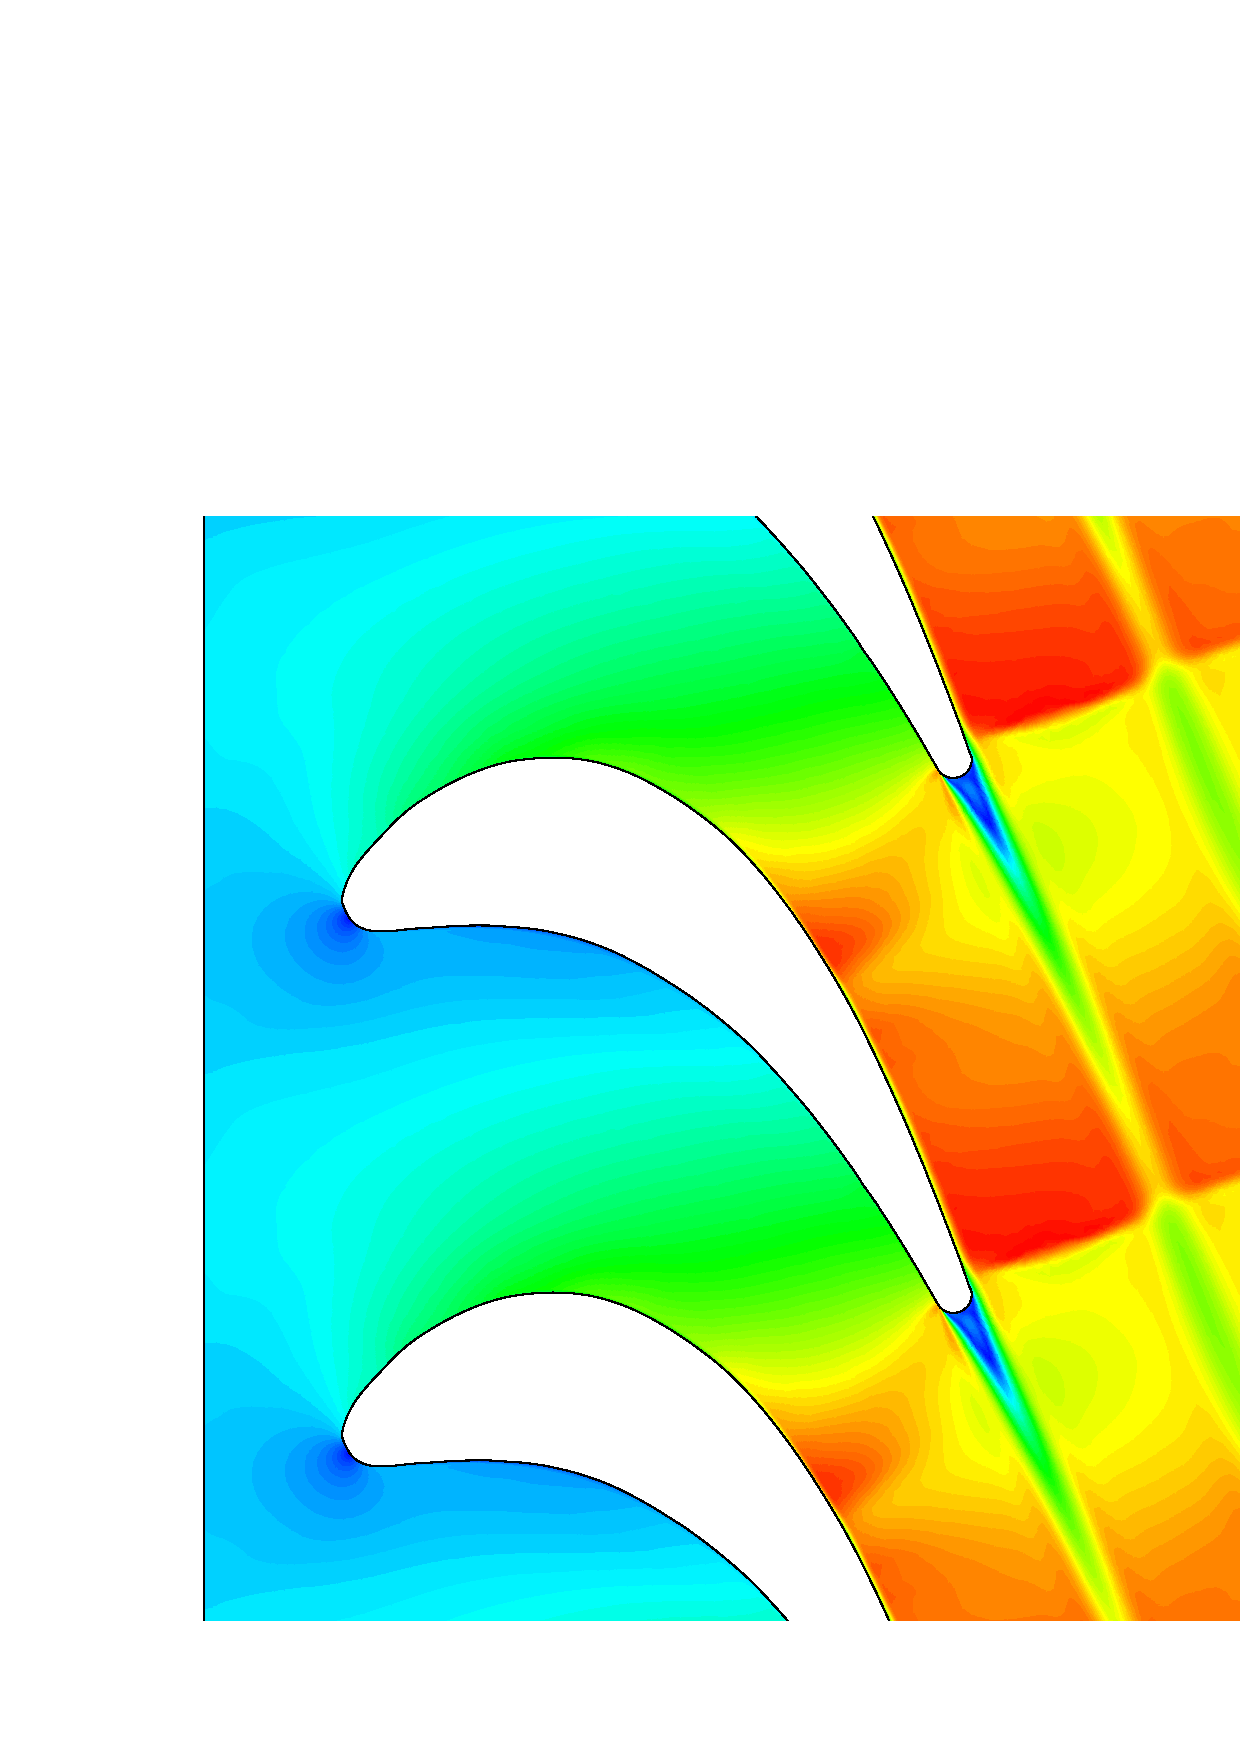
\includegraphics[width=70mm,clip=t]{CHAP_NONLIN/FIGURE/vki_mach.pdf}}
        &
    \subfigure[Particle traces near the trailing edge]
       {\fbox{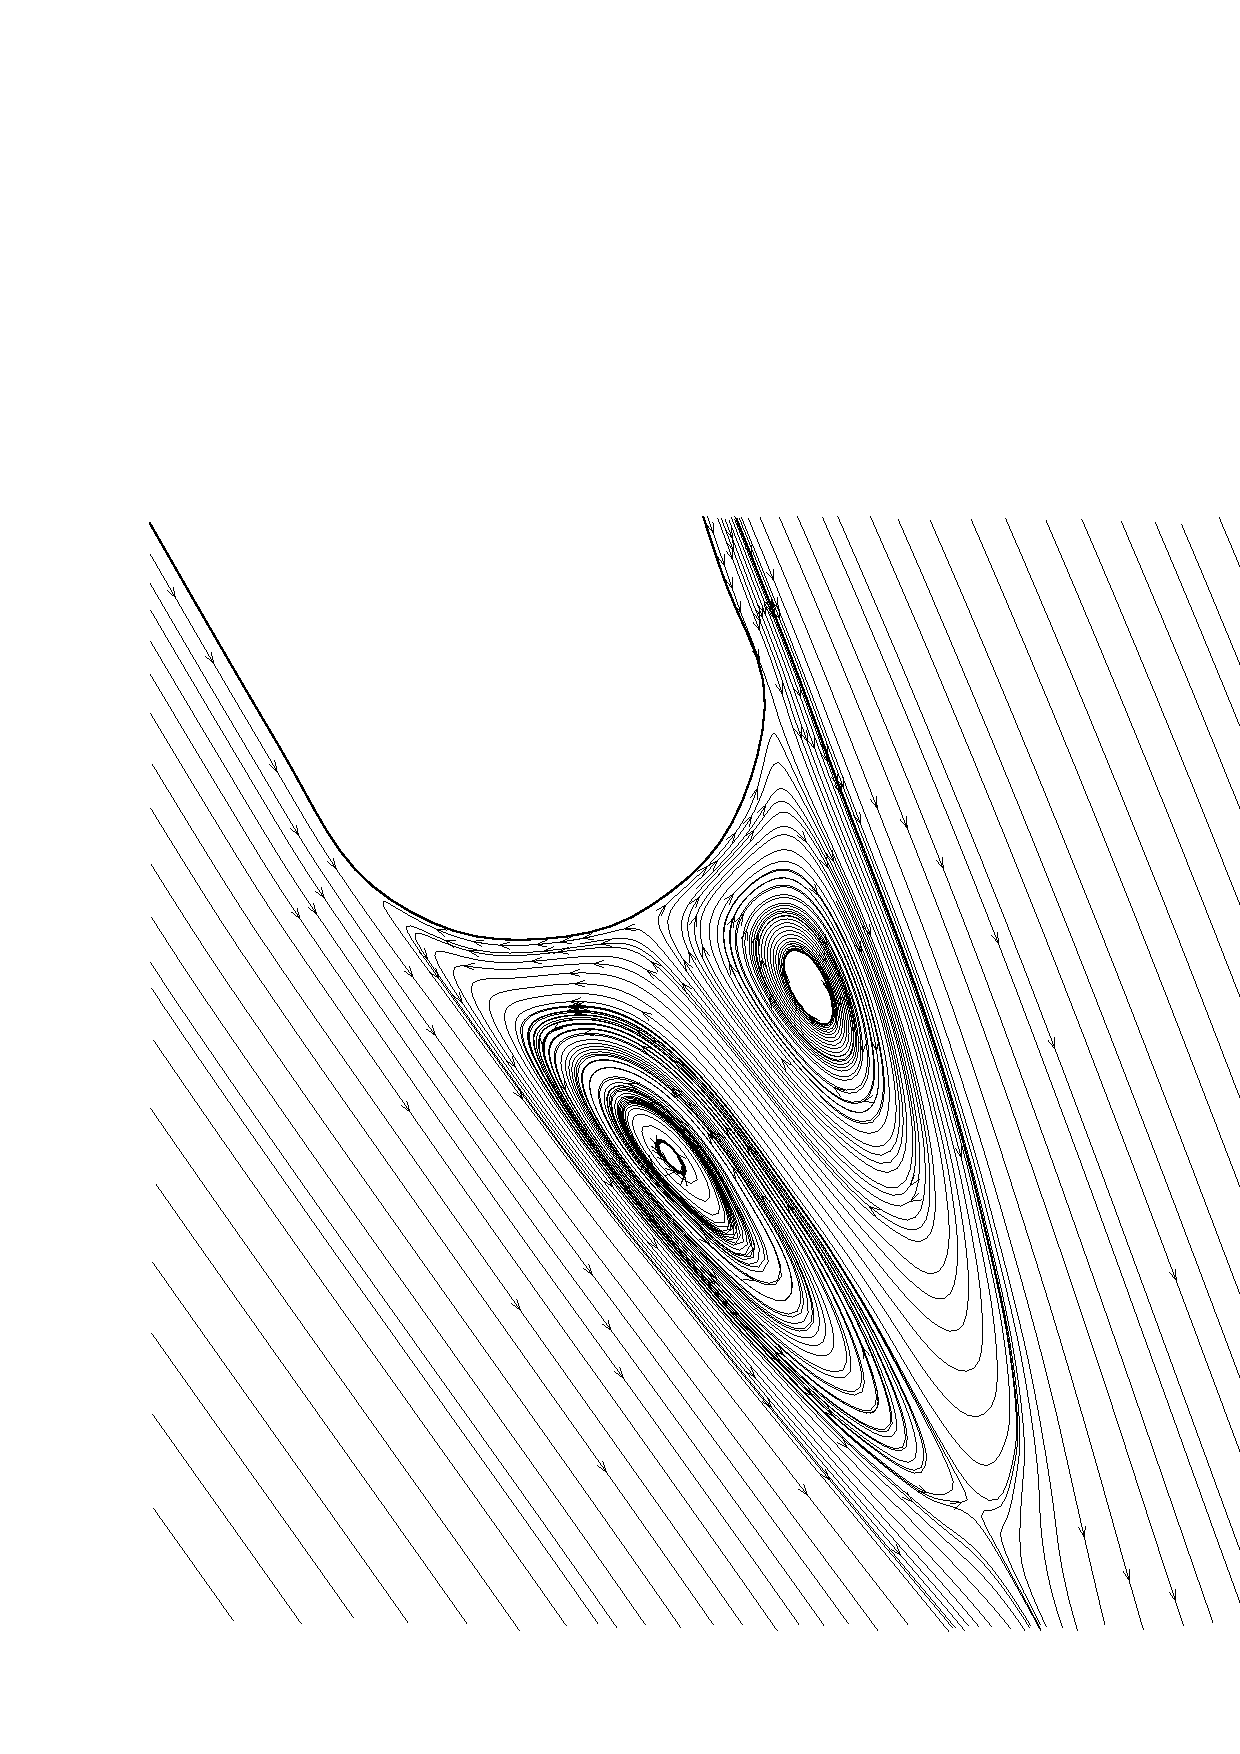
\includegraphics[width=70mm,clip=t]{CHAP_NONLIN/FIGURE/vki_traces.pdf}}}
  \end{tabular}
 \end{center}
 \vspace{-8mm}
 \caption{VKI LS59 rotor blade. $M\sm{is2} = 1$, $Re\sm{2} = 7.6\cdot10\se{5}$.
          Computed solution}
 \label{vki_mach.fig}
\end{figure}
%

 The isentropic Mach number distribution on the blade surface is given in
 Fig. \ref{vki_mach_blade.fig} for the case with an isentropic outlet Mach
 of unity. The sonic conditions are obtained at $x/c \approx 0.47$
 on the suction side and at the trailing edge in the pressure side
 resulting in fairly straight sonic line across the blade passage as
 shown in the Mach number contours of Fig. \ref{vki_mach.fig}a.
 The flow is accelerated along the suction side up to $x/c = 0.6$ followed
 by a moderate deceleration downstream.
 For this blade, the experimental data of
 Kiock et al. \citeyear{Kiock:1} include exit flow angles, inlet Mach number
 and loss coefficient defined as
 $\xi = 1 - \frac{\left|v\sm{2}\right|}{\left|v\sm{is2}\right|}$, where
 $v\sm{is2}$ represents the isentropic outlet velocity. The comparison
 between the experimental and the computed values of such quantities as a
 function of the outlet Mach number is reported in Fig. \ref{vki_blade.fig}.
%
%
\begin{figure}
 \begin{center}
  \begin{tabular}{c}
    \subfigure[Exit flow angle]
       {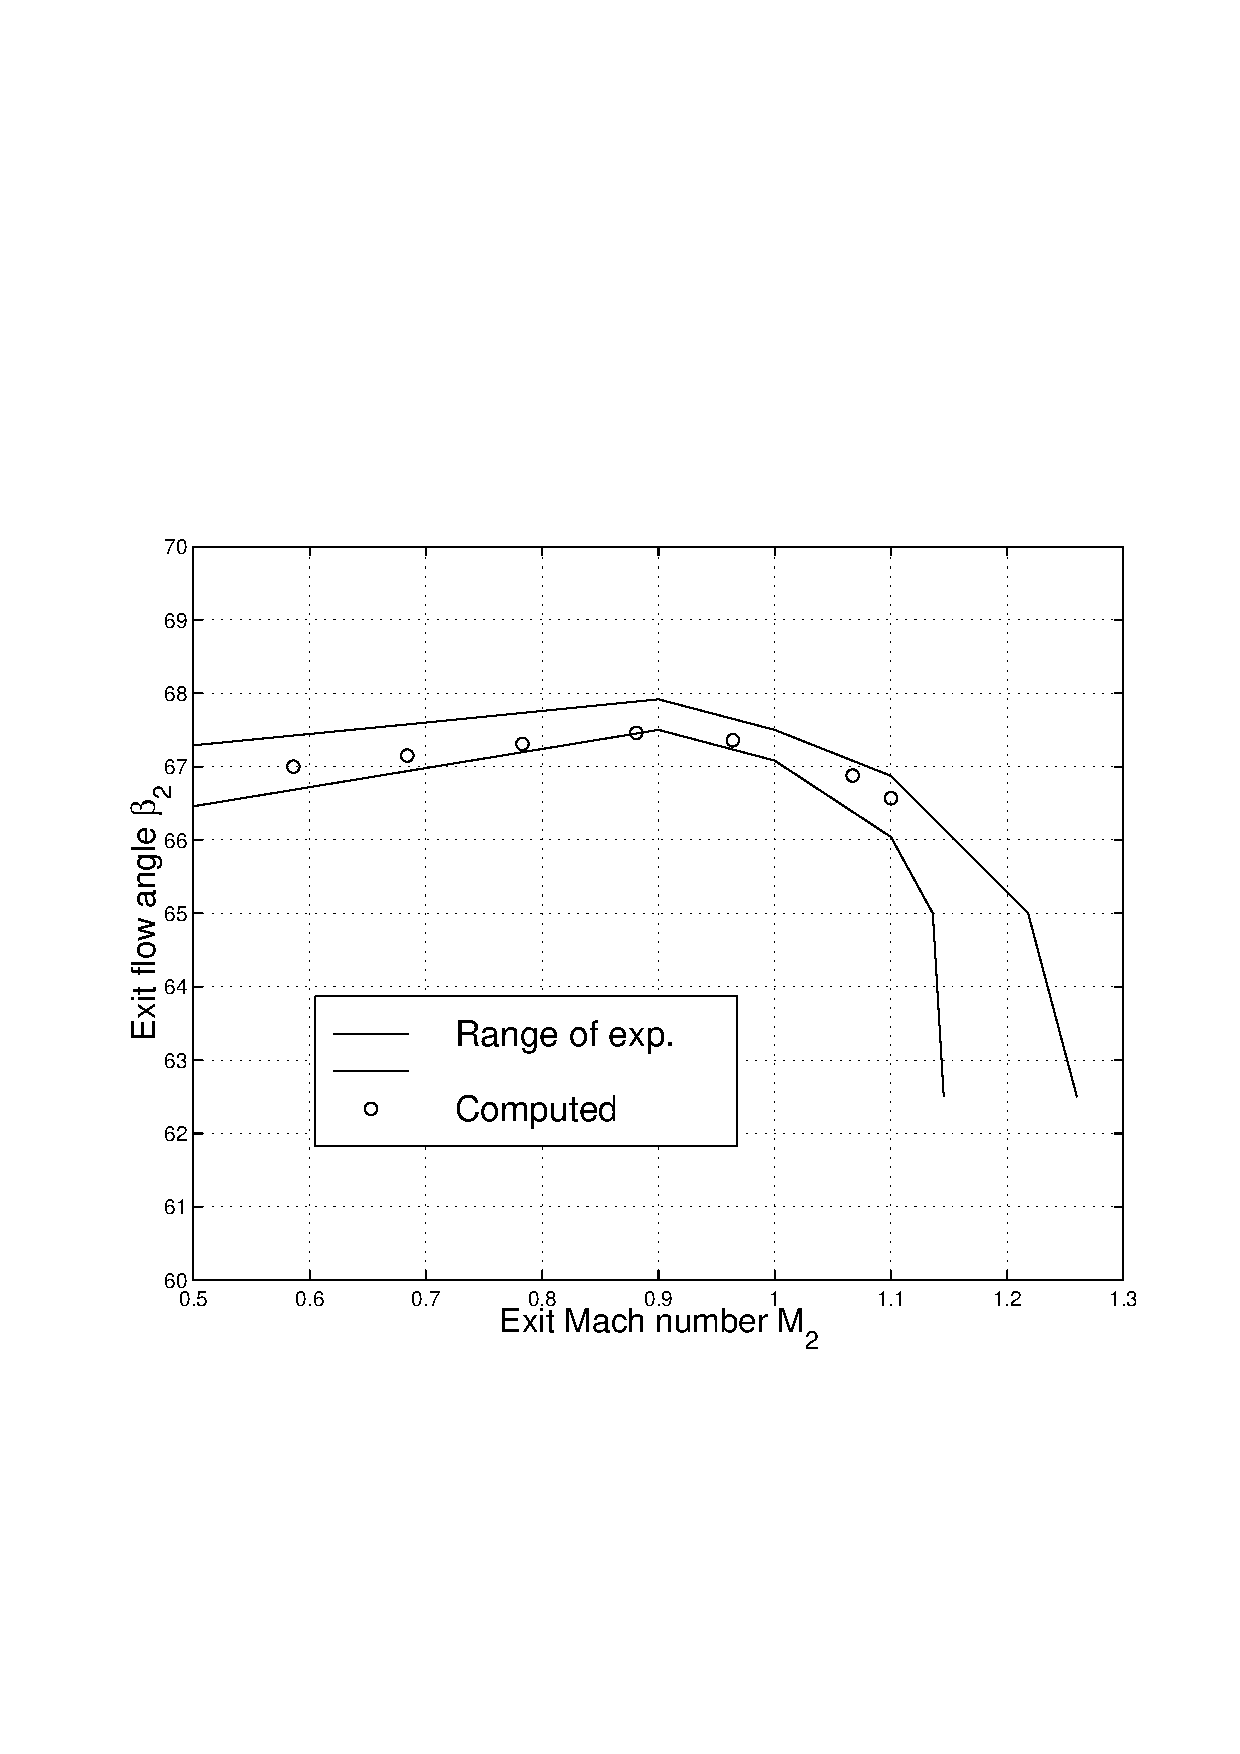
\includegraphics[width=80mm,clip=t]{CHAP_NONLIN/FIGURE/vki_beta2.pdf}}
        \vspace{-4mm}\\
    \subfigure[Inlet Mach number]
       {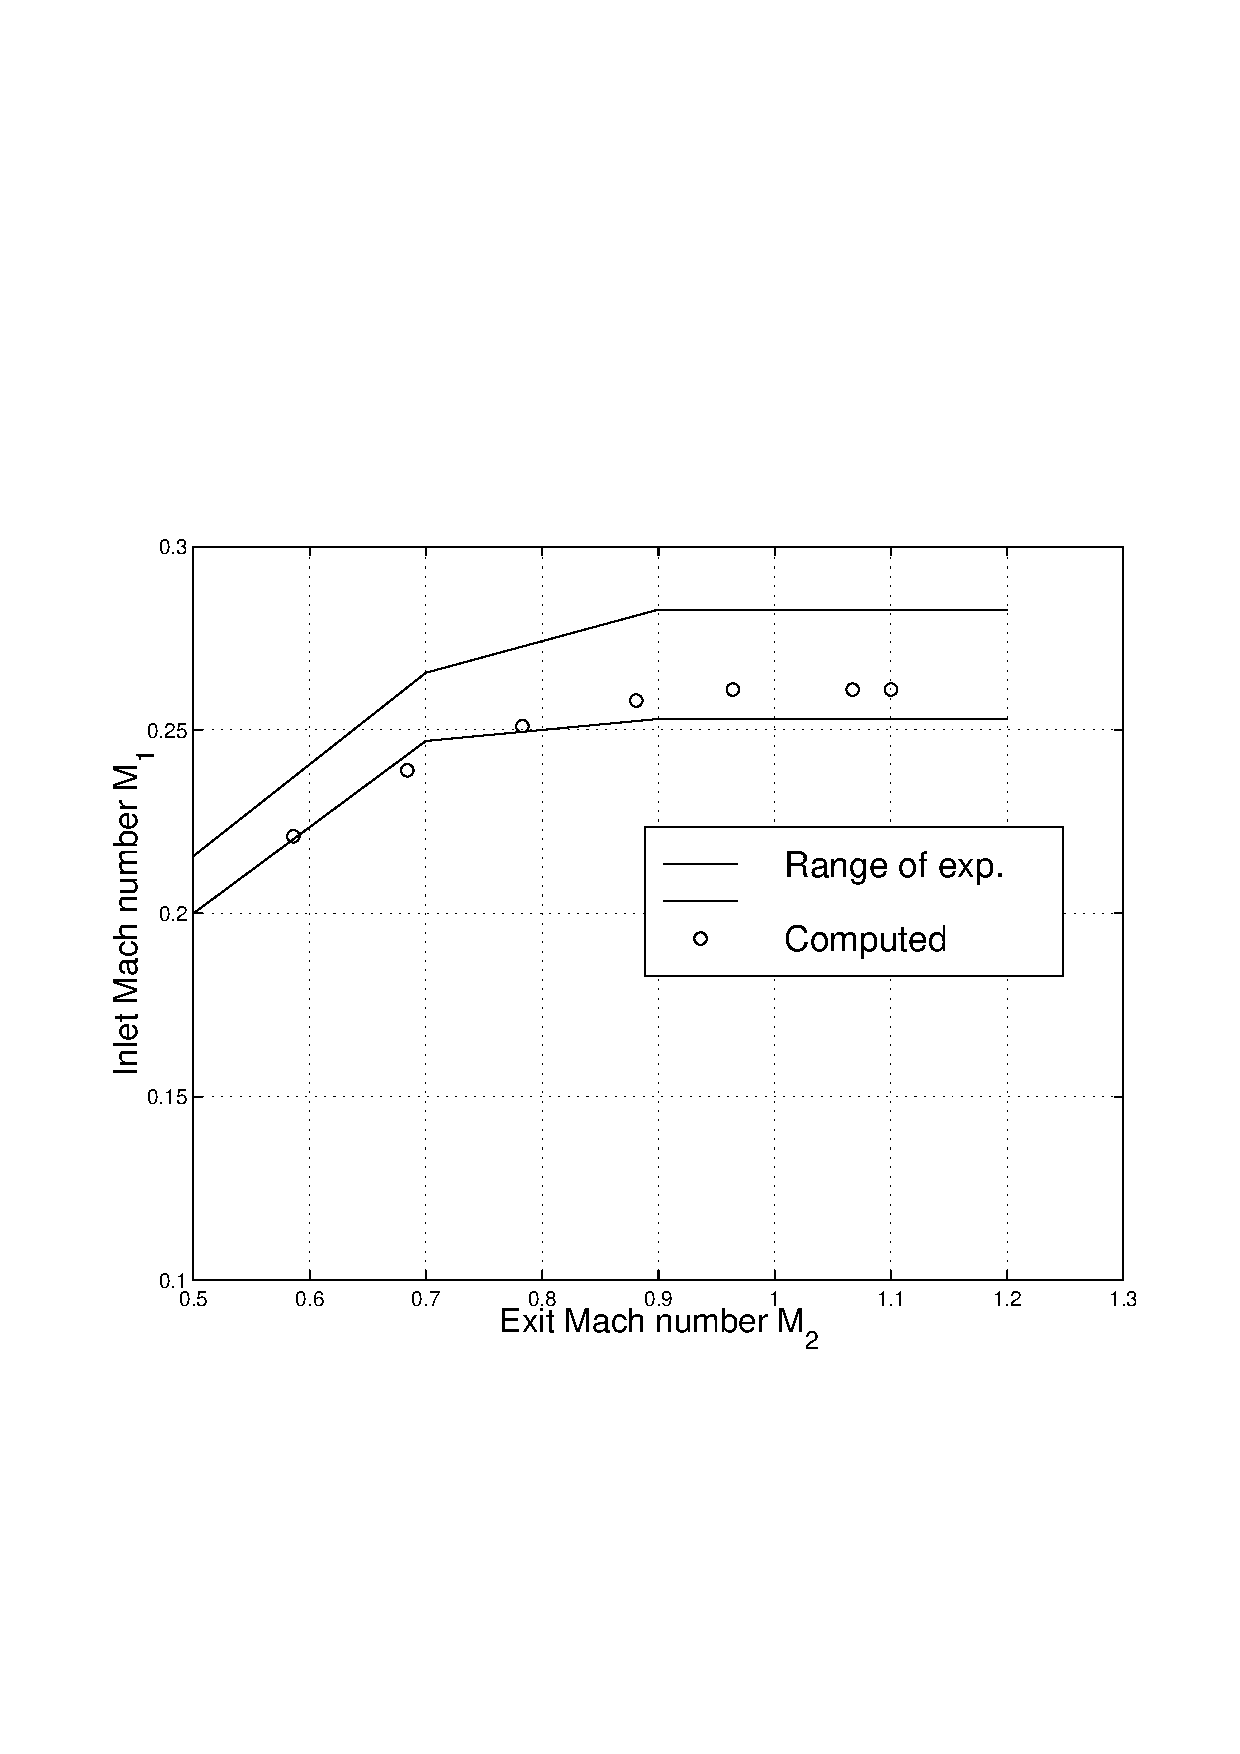
\includegraphics[width=80mm,clip=t]{CHAP_NONLIN/FIGURE/vki_mach1.pdf}}
        \vspace{-4mm}\\
    \subfigure[Loss coefficient]
       {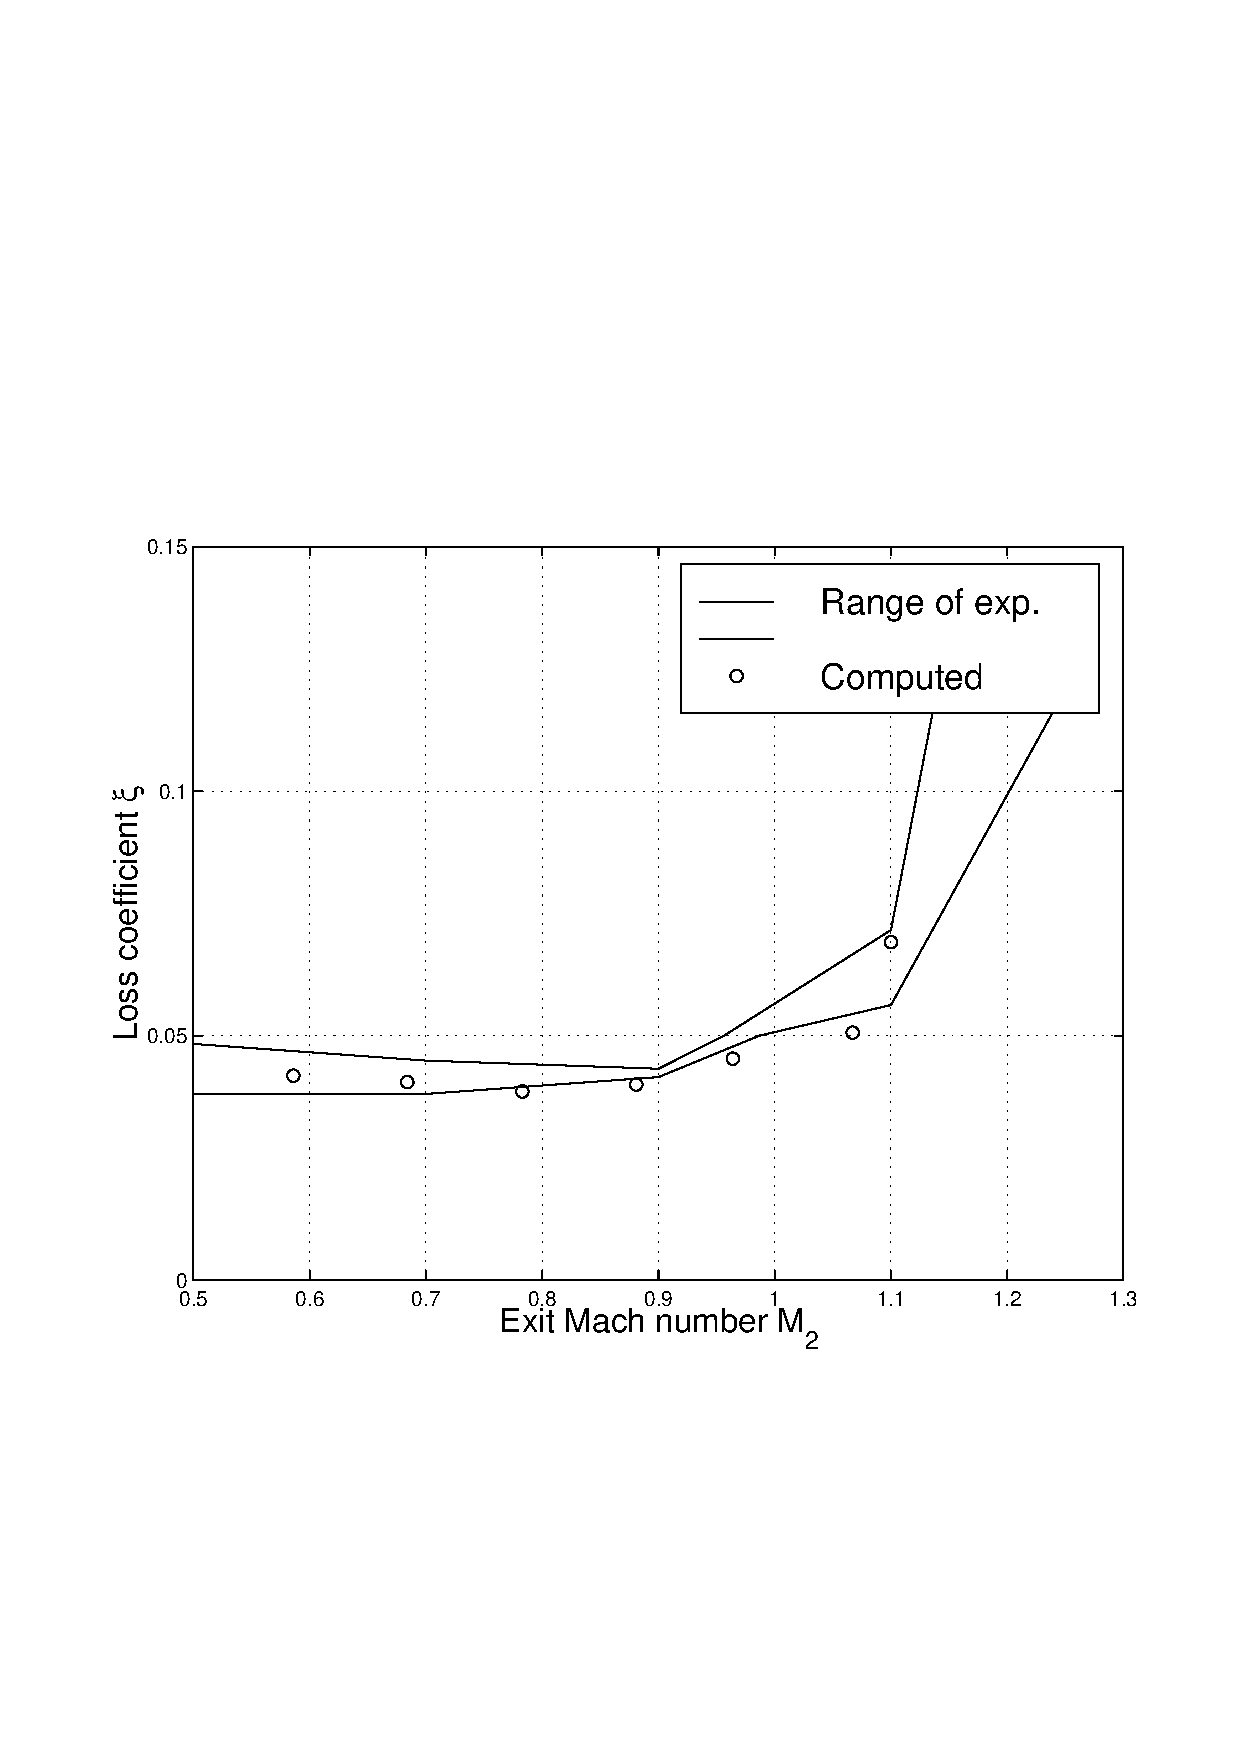
\includegraphics[width=80mm,clip=t]{CHAP_NONLIN/FIGURE/vki_loss.pdf}}
  \end{tabular}
 \end{center}
 \vspace{-8mm}
 \caption{VKI LS59 rotor blade. Computed solutions}
 \label{vki_blade.fig}
\end{figure}
%
%

 Fig. \ref{vki_res.fig} compares the convergence history obtained using the
 line-implicit solver of Appendix \ref{multigrid.chap}, on a single grid and
 on four grid W-type cycle. The convergence history
 of a single grid, point-Jacobi, iterative implicit scheme as the one
 used by Sayma et al. \citeyear{Luca:10}, is also plotted.
 It is evident that the single grid solution is not converged
 and the reason of this could be blamed to the grid anisotropy as well as
 to the blunt trailing edge of the blade which causes a recirculation bubble
 which could be inherently unsteady (Fig. \ref{vki_mach.fig}b).
 The single grid implicit scheme of Sayma et al. \citeyear{Luca:1} converges very slowly
 because not designed to be effective in damping error arising from highly stretched
 meshes.
%
\begin{figure}
 \centerline{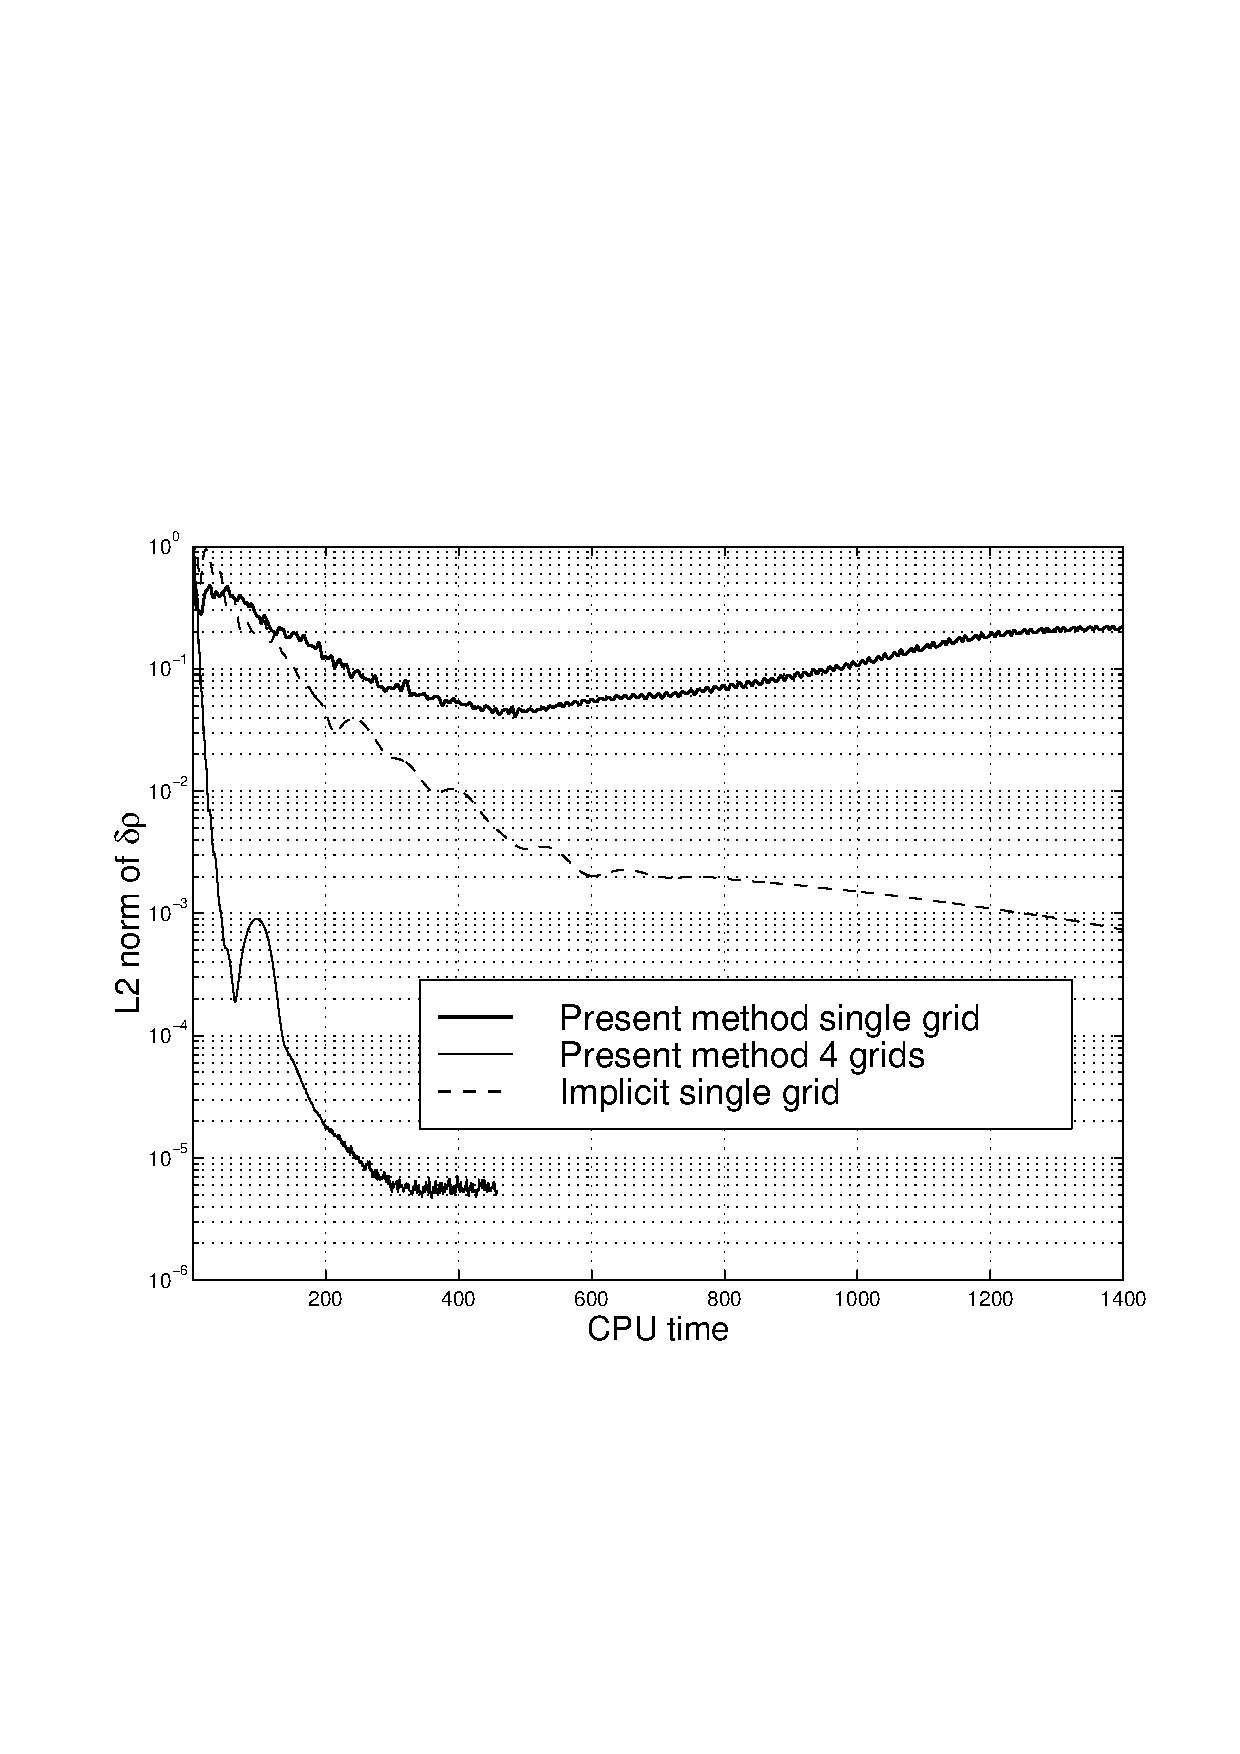
\includegraphics[width=130mm,clip=t]{CHAP_NONLIN/FIGURE/vki_res.pdf}}
 \caption{VKI LS59 rotor blade. Residual history}
 \label{vki_res.fig}
\end{figure}
%
